\newgeometry{bottom=0.1cm}
\chapter*{Program GazeSwitch}
\label{rozdz6}

Praca stanowi projekt zaliczeniowy z przedmiotu Programowanie Zaawansowane FM i NI na Wydziale Fizyki Uniwersytetu Warszawskiego. W ramach projektu napisano program \textbf{GazeSwitch}. Jest to program wykorzystujący sygnał okulograficzny do detekcji spojrzenia w wybranym kierunku. Program wykorzystuje narzędzia i metody cyfrowego przetwarzania obrazu. Sygnał, czyli pojedyńcze klatki strumienia filmowego przesyłanego przez okulograf jest analizowany w programie GazeSwitch. Podstawowym elementem programu jest \textbf{algorytm detekcji spojrzenia}. Efektem działania algorytmu jest klasyfikacja sygnału do jednego z dwóch zbiorów -- detekcja spojrzenie w kierunku jednej z diód lub brak spojrzenia w tym kierunku. Klasyfikacja sygnału do zbioru odpowiadającego spojrzeniu na jedną z diód wyzwala odpowiedź przesyłaną do graficznego interfejsu użytkownika. Efekt jaki wywołuje przesłana odpowiedź zależy od miejsca wykonywania w jakim znajduje się graficzny interfejs użytkownika

\section{Ogólna struktura programu GazeSwitch}

Do akwizycji sygnału okulograficznego wykorzystano urządzenie przedstawione na ilustracji \ref{fig1}

\begin{figure}[h!]
\centering
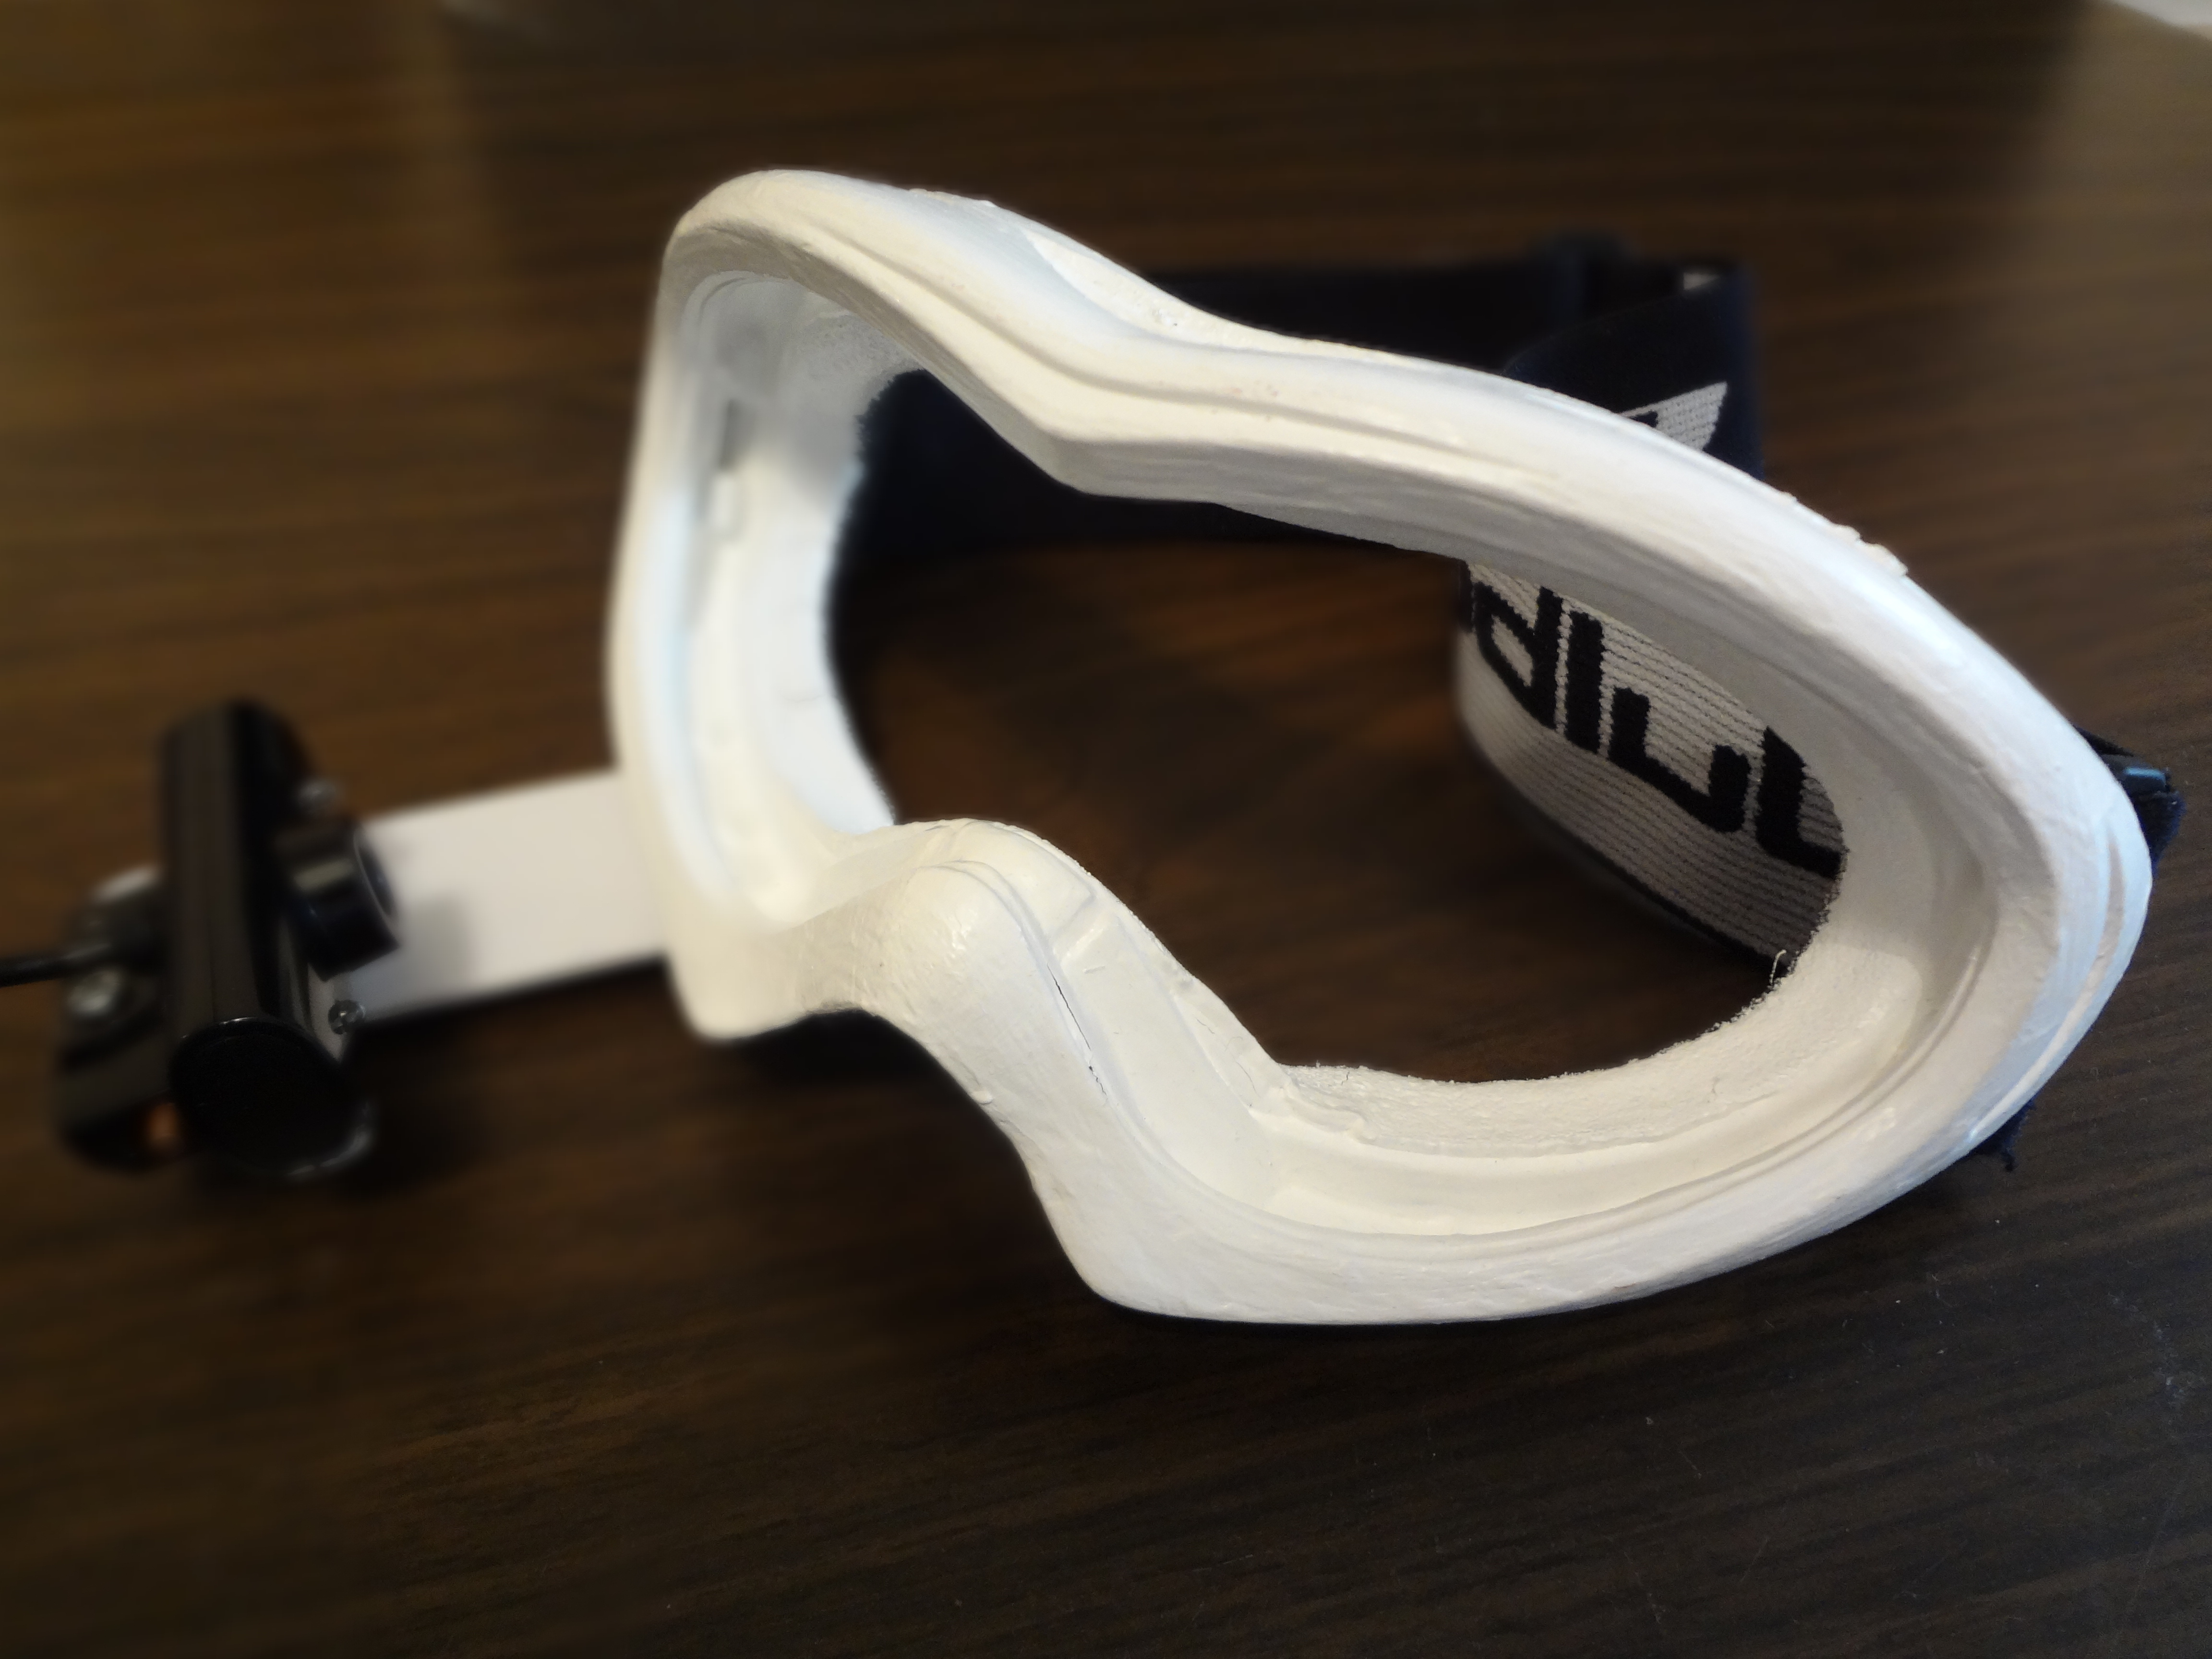
\includegraphics[scale=0.04]{images/1.jpg}
\caption{Okulograf wykorzystywany przy pisaniu programu. \label{fig1}}
\end{figure}

\newpage
Sygnał zbierany przez prosty okulograf i analizowany przez program GazeSwitch jest przekazywany do graficznego interfejsu użytkownika (GUI). Szkic działania prezentuje ilustracja \ref{fig2}.
\begin{figure}[!h]
\centering
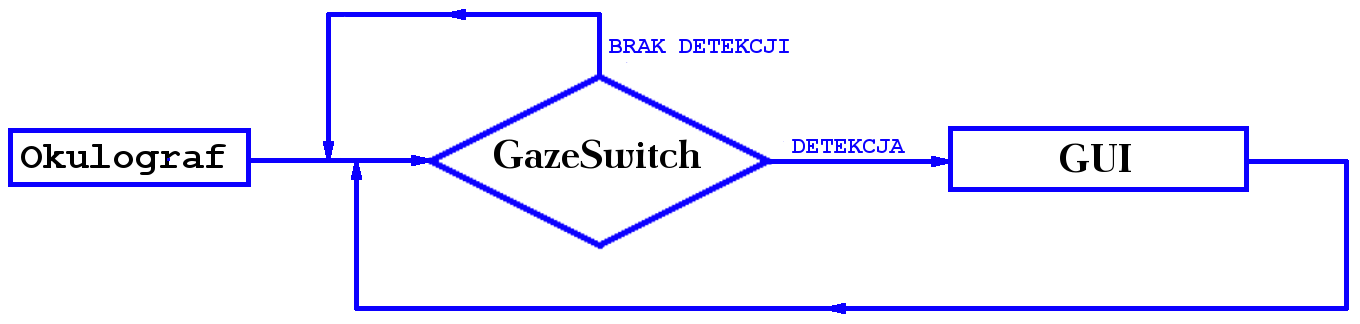
\includegraphics[scale=0.3]{images/2.png}
\caption{Schemat blokowy działania systemu. \label{fig2}}
\end{figure}

\section{Ogólna struktura algorytmu detekcji spojrzenia}
Algorytm detekcji spojrzenia jest oparty na podstawowych metodach cyfrowego przetwarzania obrazu (DIP; ang. \textit{digital image processing}).

\begin{wrapfigure}{o}{0.5\textwidth}
  \vspace{-0.3cm}
  \begin{center}
    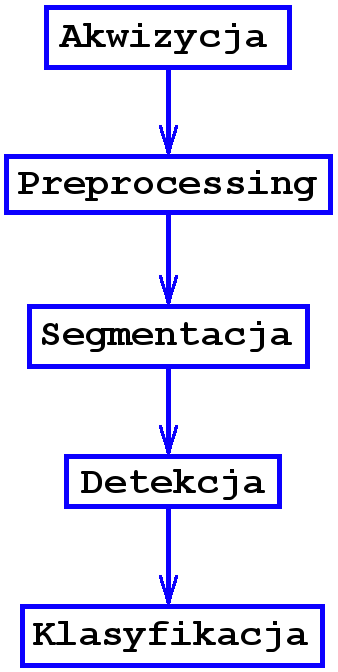
\includegraphics[scale=0.3]{images/3.png}
  \end{center}
  \caption{Ogólna struktura algorytmu detekcji spojrzenia w programie GazeSwitch. \label{fig3}}
\end{wrapfigure}

W algorytmie detekcji spojrzenia, wykorzystywanym przez program GazeSwitch można wyróżnić pięć podstawowych etapów przetwarzania obrazu oka. Schematycznie algorytm przedstawia ilustracja \ref{fig3}. Pierwszy etap stanowi akwizycja obrazu, czyli jego przechwycenie. Drugi etap to przetwarzanie wstępne przygotowujące obraz do obróbki właściwej. W trzecim etapie z obrazu wyodrębnione zostają określone obszary. Czwarty etap stanowią obliczenia wykonywane na wyodrębnionych obszarach, a piąty to przeprowadzona na podstawie obliczeń klasyfikacja. Algorytm wykonuje powyższe kroki na każdej klatce strumienia wideo.

Schemat działania algorytmu na konkretnej klatce strumienia przedstawia ilustracja \ref{fig4}.
\newpage
\restoregeometry
\begin{figure}[!h]
\centering
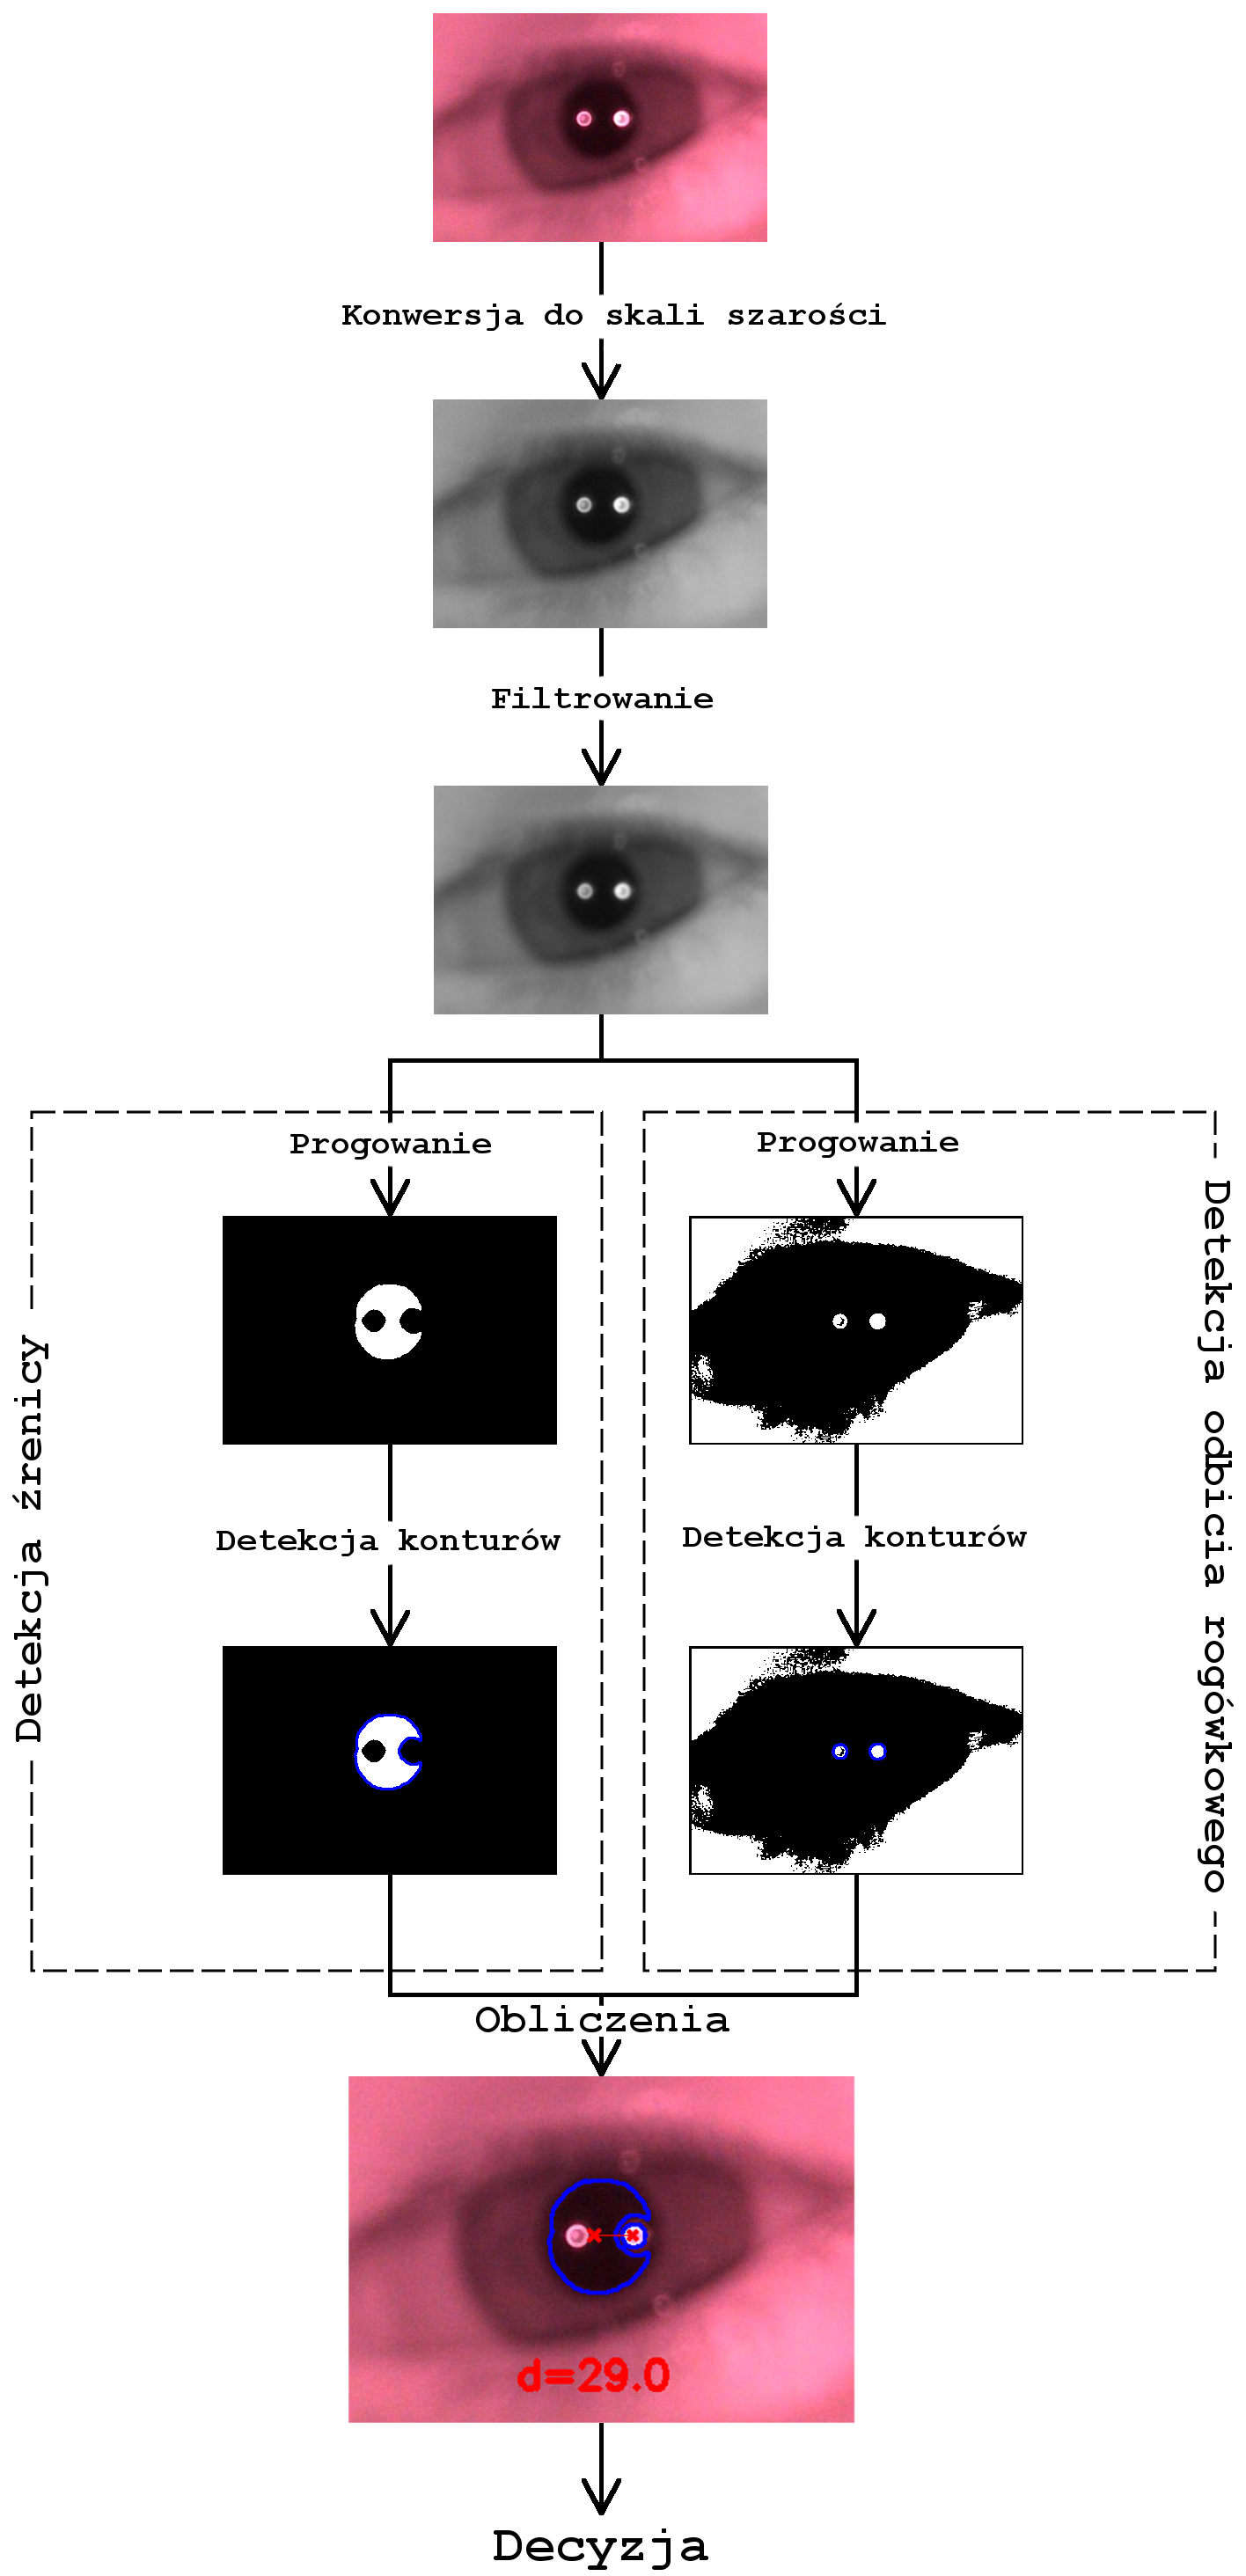
\includegraphics[scale=0.2]{images/4.png}
\caption{Schemat działania algorytmu detekcji źrenicy. \label{fig4}}
\end{figure}

\newpage
\restoregeometry
\section{Szczegóły implementacji}
Działanie poszczególnych etapów algorytmu przedstawiane jest na reprezentatywnym obrazie \ref{fig5}.

\begin{figure}[!h]
\centering
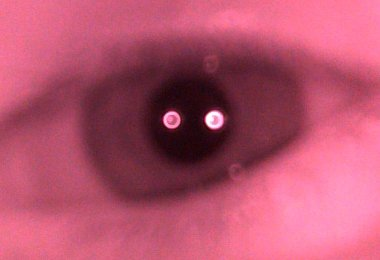
\includegraphics[scale=0.3]{images/5.jpg}
\caption{Reprezentatywny obraz oka. \label{fig5}}
\end{figure}

\subsection{Preprocessing}
Preprocessing inaczej nazywany przetwarzaniem wstępnym obejmuje nazwą wszystkie operacje wykonywane na obrazie w celu przygotowania go do obróbki właściwej. W algorytmie detekcji spojrzenia do tego etapu można zaliczyć konwersje obrazu do skali szarości oraz filtrowanie.
\subsubsection{Konwersja obrazu do skali szarości}
Konwersje do obrazu monochromatycznego wykonano zgodnie ze wzorem \ref{eq1}. Efekt przedstawia ilustracja \ref{fig6}

\begin{equation}
  \centering
  GY = 0.299\cdot R + 0.587\cdot G + 0.144\cdot B \label{eq1}
\end{equation}
  

\begin{figure}[!h]
\centering
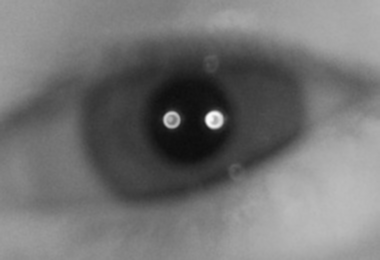
\includegraphics[scale=0.25]{images/6.png}
\caption{Obraz w skali szarości. \label{fig6}}
\end{figure}

\newpage
\loadgeometry{highPage}
\subsubsection{Filtrowanie}
Filtrowanie jest operacją mającą na celu pozbycie się szumu z obrazu. W szczególności filtry wygładzające są stosowane w celu zmniejszenia wariancji wartości pikseli. W algorytmie został zastosowany filtr gaussowski z jądrem 7x7. Efekt działania filtru wyraźny staje się dopiero po przeprowadzeniu segmentacji będącej następnym omawianym w pracy etapem przetwarzania. Rysunek \ref{fig7} efekt ten ilustruje.

\begin{figure}[h!]
  \begin{subfigure}[h!]{0.3\textwidth}\subcaption{\label{fig7a}}
    \centering
    
\includegraphics[scale=0.4]{images/7.png}
  \end{subfigure}\hspace{2.5cm}
  \begin{subfigure}[h!]{0.3\textwidth}\subcaption{\label{fig7b}}
    \centering
    
\includegraphics[scale=0.4]{images/8.png}
  \end{subfigure}
  \caption{{a)} Obraz poddany segmantacji bez poprzedzającej go filtracji, {b)} Obraz poddany segmantacji po uprzedniem przefiltrowaniu. \label{fig7}}
\end{figure}

\subsection{Segmentacja}
Segmentacja jest najprostszą metodą klasyfikacji. Ze względu jednak na znaczną rolę jaką odgrywa w algorytmie detekcji spojrzenia została ona wyodrębniona jako odzielny etap. Segmentacja jest podziałem obrazu na spójne fragmenty. Polega na wyodrębnieniu z obrazu określonych obszarów, a następnie zaklasyfikowaniu każdego z pikseli do jednego z tych obszarów. W wyniku segmentacji obraz zostaje podzielony na obszar zainteresowania (ROI, ang. \textit{Region Of Interest}) oraz tło. Do segmentacji zastosowano metodę progowania binarnego, czyli jedną z metod konwersji obrazu z gradacją szarości do obrazu binarnego (biało-czarnego). Efekt progowania ilustruje rysunek \ref{fig8}.

\begin{figure}[h!]
  \begin{subfigure}[h!]{0.3\textwidth}\subcaption{\label{fig8a}}
    \centering
    
\includegraphics[scale=0.4]{images/9.png}
  \end{subfigure}\hspace{2.5cm}
  \begin{subfigure}[h!]{0.3\textwidth}\subcaption{\label{fig8b}}
    \centering
    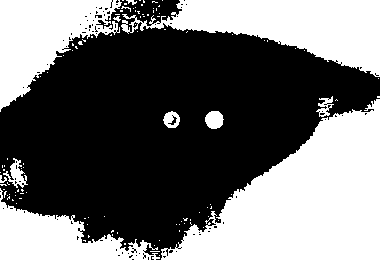
\includegraphics[scale=0.4]{images/10.png}
  \end{subfigure}
  \caption{Efekt progowania obrazu {a)} przy detekcji konturu źrenicy, {b)} przy detekcji konturów odbić od rogówki. \label{fig8}}
\end{figure}

\newpage
\subsection{Detekcja}
Chociaż metody segmentacji pozwalają na wyodrębnienie z obrazu określonych obszarów nie przynoszą one żadnej o nich ilościowej informacji. Następnym krokiem jest sprowadzenie tych obszarów do konturów -- obiektów geometrycznych mogących być ilościowo opisywanymi. Kontur jest zbiorem punktów reprezentujących na obrazie krzywą. W algorytmi detekcji spojrzenia do konturyzacji wykorzystano funkcję biblioteki \textit{openCV} o nazwie \textit{cv2.findContours()}. Funkcja jest implementacją algorytmu opisanego w pracy Teh, C., and R.T. Chin. “On the Detection of Dominant Points on Digital Curves.”. Na wejście funkcja przyjmuje obraz binarny, a na wyjście przekazuje w strukturze drzewiastej obliczone kontury. Efekt działania funkcji \textit{cv2.findContours()} przedstawia ilustracja \ref{fig9}.

\begin{figure}[h!]
  \begin{subfigure}[h!]{0.3\textwidth}\subcaption{\label{fig9a}}
    \centering
    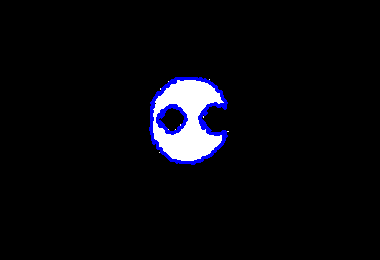
\includegraphics[scale=0.48]{images/11.png}
  \end{subfigure}\hspace{2.5cm}
  \begin{subfigure}[h!]{0.3\textwidth}\subcaption{\label{fig9b}}
    \centering
    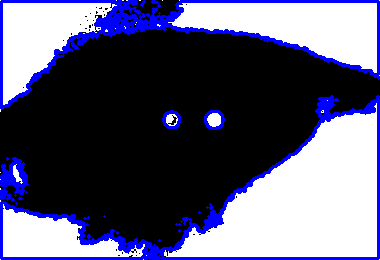
\includegraphics[scale=0.48]{images/12.png}
  \end{subfigure}
  \caption{Efekt działania funkcji \textit{cv2.findContours} {a)} przy detekcji konturu źrenicy, {b)} przy detekcji konturów odbić od rogówki. \label{fig9}}
\end{figure}

\subsection{Klasyfikacja}

Kontury są obiektami geometrycznymi i jak wszystkie obiekty geometryczne posiadają swoje charakterystyki, a w tym i momenty. Momenty są wielkościami opisującymi kształt figury. W przypadku dyskretnym opisane są wzorem ogólnym \ref{eq2}:

\begin{equation}
  m_{ij}=\sum_{x,y}\Big(obraz(x,y)\cdot x^{i}\cdot y^{j}\Big)\label{eq2}
\end{equation}

\newpage
Rzędem momentu nazywa się wielkość (i+j). Moment rzędu 0 wyraża się wzorem \ref{fig10}:
\begin{equation}
  m_{00}=\sum_{x,y}\Big(obraz(x,y)\Big)\label{fig10}
\end{equation}
i jest ilością pikseli zawierających się w konturze, będąc tym samym proporcjonalnym do pola jego powierzchni. W celu klasyfikacji na wykryte kontury nakładane są odpowiednie warunki. Kontur źrenicy jest jedynym znacząco dużym obszarem zaciemnienia na obrazie. Dla poprawnego działania algorytmu wystarczy więc zgrubne nałożenie od dołu warunku na wielkość powierzchni konturu:
\begin{enumerate}
\item $\displaystyle m_{00}\  \geq\  \textit{próg}_{\textit{Ź}}$.
\end{enumerate}
Na kontur reprezentujący odbicie rogówkowe nałożone zostały trzy warunki. Pierwszy dotyczy pola powierzchni, dwa pozostałe kolistego kształtu konturu:
\begin{enumerate}
\item $\displaystyle m_{00}\  \geq\  \textit{próg}_{\textit{R}}$.
\item $\displaystyle \lvert1-\frac{m_{00}}{\pi\cdot (\frac{w}{2})^{2}}\rvert\  \leq\  0.2$,
gdzie: $w$ - szerokość prostokąta opisanego na konturze.
\item $\displaystyle \lvert1 - \frac{w}{h}\rvert\  \leq\  0.2$,
gdzie: $h$ - wysokość prostokąta opisanego na konturze.
\end{enumerate}   
Efekt klasyfikacji przedstawia ilustracja \ref{fig11}
\begin{figure}[h!]
  \begin{subfigure}[h!]{0.3\textwidth}\subcaption{\label{fig11a}}
    \centering
    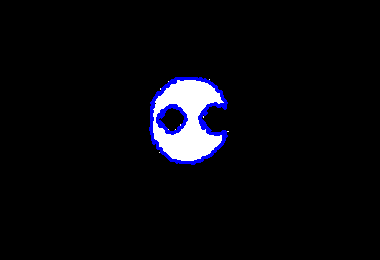
\includegraphics[scale=0.48]{images/11.png}
  \end{subfigure}\hspace{2.5cm}
  \begin{subfigure}[h!]{0.3\textwidth}\subcaption{\label{fig11b}}
    \centering
    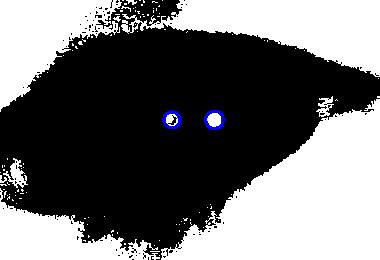
\includegraphics[scale=0.48]{images/13.png}
  \end{subfigure}
  \caption{Efekt działania funkcji \textit{cv2.findContours} {a)} przy detekcji konturu źrenicy, {b)} przy detekcji konturów odbić od rogówki. \label{fig11}}
\end{figure}

Współrzędne środka konturu reprezentującego źrenicę oraz współrzędne środka konturu reprezentującego odbicie rogówkowe są następnie podawane na wejście funkcji decyzyjnej.
\subsection{Funkcja decyzyjna}
Funkcja na podstawie współrzędnych środka źrenicy i odbicia rogówkowego liczy odległość zgodnie ze wzorem:
\begin{equation}
  d(\textit{Ź},R) = \sqrt{\Big(X_{\textit{Ź}} - X_{R}\Big)^{2} + \Big(Y_{\textit{Ź}} - Y_{R}\Big)^{2}},
\end{equation}

gdzie: $X_{\textit{Ź}}, X_{\textit{R}}$ -- współrzędna horyzontalna środka źrenicy i odbicia rogówkowego, $Y_{\textit{Ź}}, Y_{\textit{R}}$ -- współrzędna wertykalna środka źrenicy i odbicia rogówkowego.

Efekt obliczeń na obrazie reprezentacyjnym przedstawia ilustracja \ref{fig12}
\begin{figure}[h!]
  \begin{subfigure}[h!]{0.3\textwidth}\subcaption{\label{fig12a}}
    \centering
    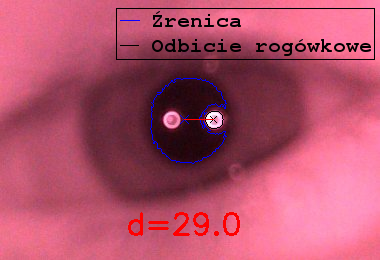
\includegraphics[scale=0.5]{images/14.png}
  \end{subfigure}\hspace{2.5cm}
  \begin{subfigure}[h!]{0.3\textwidth}\subcaption{\label{fig12b}}
    \centering
    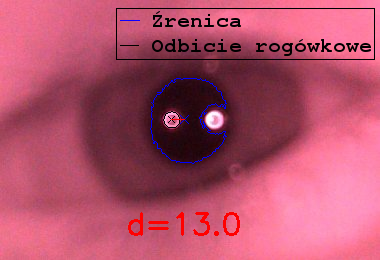
\includegraphics[scale=0.5]{images/15.png}
  \end{subfigure}
  \caption{Efekt obliczeń {a)} przy detekcji odbicia rogówkowego od lewej diody, {b)} przy detekcji odbicia rogówkowego od prawej diody. \label{fig12}}
\end{figure}

Następnie w zależności od zadanego progu funkcja przyjmuje warość pobudzenie lub brak pobudzenia.

\[ Funkcja\ decyzyjna\ = \left\{
  \begin{array}{l l}
    pobudzenie & \quad dla \ \ min\Big(d(\textit{Ź},R)\Big) \le \textit{próg}\\
    brak\ pobudzenia & \quad w\ przeciwnym\ razie
  \end{array} \right.\]

Jeżeli funkcja decyzyjna przyjmie wartość pobudzenie określoną ilość razy pod rząd do GUI zostaje przesłana informacja o pobudzeniu. Efekt pobudzenia zależy od miejsca wykonywania, w którym znajduje się GUI.

\newpage
\subsection{Struktura katalogu}
W katalogu głównym znajdują się cztery pliki źródłowe:
\begin{itemize}
\item \textit{gazeSwitch.cpp}
\item \textit{show.cpp}
\item \textit{steps.cpp}
\item \textit{save.cpp}
\end{itemize}

Plik \textit{gazeSwitch.cpp} to docelowy program. Plik \textit{show.cpp} na strumień wideo nanosi efekt działania algorytmu detekcji źrenicy i tak przetworzone obrazy wyświetla na monitorze. Plik \textit{steps.cpp} to program, który prezentuje kroki algorytmu na przykładowym obrazie podanym jako argument linii komend. Plik \textit{save.cpp} zapisuje w plikach graficznych efekt działania algorytmu detekcji spojrzenia na poszczególnych klatkach strumienia filmowego.

Do kompilacji wykorzystano CMake (Cross-platform Make) - narzędzie do automatycznego zarządzania procesem kompilacji programu. Komunikację z interfejsem użytkownika zaimplementowano w biblitece ZeroMQ (asynchroniczna biblioteka do realizacji komunikacji w środowisku rozproszonym). Zastososowano protokół nadawca-odbiorca. Program uruchomiono w systemie Linux.
